%%
%% Author: thompson
%% 25.11.17
%%

% Preamble
\documentclass[11pt]{article}

% Packages
\usepackage{a4wide}
\usepackage[ngerman]{babel}
\usepackage[utf8]{inputenc}

\usepackage{scrextend}
\usepackage{enumerate}
\usepackage{graphicx}


% Document
\begin{document}

    \graphicspath{{PictureDoc/}}


    \section{OMNeT++}
    \subsection{Q\&A}

    \begin{enumerate}[\thesubsection .1]
        \item Wie wird eine Topologie erstellt und dessen Funktionalität realisiert?\\
        Eine Topologie, sprich eine Simulation wird in OMNeT++ mithilfe mehrerer Datentypen definiert. Es gibt:
        \begin{enumerate}[$\circ$]
            \item .NED - \textbf{NE}twork \textbf{D}escription File
            In diesen beschreibt man, wie der Name bereits verät, das Netzwerk mit all dessen Knoten, Empfängern wie Sendern.
            Neben den DataNodes beschreibt man auch den groben Funktionsumfang, etwa wann Daten gesendet werden sowie Delay.
            Mithilfe 2er Modi: Source und Design lässt sich das Netzwerk graphisch als auch programmiertechnisch beliebig anpassen
            \item .CC - C++ Datensätze
            In diesen beschreibt man die Subfunktionen e.g. das Verhalten aller Instanzen innerhalb des Netzwerkes.
            Für gewöhnlich bedient man sich vordefinierten Spezifikationen wie cMessage oder cSimpleModule, von welchen
            die eigenen Klassen erben.
            \item .INI - Initialisierungsdatei
            Diese beschreibt das zu simulierende Netzwerk, definiert im .NED-File.
            \emph{Es gilt die Klasse anzugeben, nicht den Dateinamen.}
        \end{enumerate}

        \item Wie kompiliert und startet eine Simulation?\\
        Prinzipiell mithilfe des RUN-Buttons der IDE.

        Für gewöhnlich gilt es mithilfe von cpp-makemake ein File zu erstellen, welches dann ausgeführt wird.
        Dieses orientiert sich an der jeweiligen omnetpp.ini-Datei, worin die auszuführenden Daten spezifiziert sind.
        Ähnlich einer Kettenreaktion wird dann der Rest ausgelesen, kompiliert und ausgeführt.

        \item Wie fügt man folgende hinzu:
        \begin{addmargin}[1em]{1em}
            - Graphische Elemente: \\

            Üblicherweise mithilfe der .ned-Datei realisiert.
            Hierbei wird der TicToc mittels des network Blocks als Netzwerk
            gekennzeichnet.\\

            - Ausgaben zur Fehlersuche: \\

            Ausgaben werden wie folgt eingefügt:

            einfachste Form:
            -> EV << "Sending initial message";\\



            - Zustandsvariablen: \\

            Werden innerhalb einer Klasse definiert.

            private:
            int counter

            - (Zufällige) Parameter:

            - über die Parameter eines Moduls können zufällig
            generierte Werte zurückgegeben werden
            - um diese Werte verwenden zu können, werden sie innerhalb der
            handleMessage() eingelesen

            Beispiel:

            // The "delayTime" module parameter can be set to values like
            // "exponential(5)" (tictoc7.ned, omnetpp.ini), and then here
            // we'll get a different delay every time.
            -simtime_t delay = par("delayTime");
            -EV << "Message arrived, starting to wait " << delay << " secs...\n";
            -tictocMsg = msg;
            -scheduleAt(simTime()+delay, event);

            - die Parameter werden in omnetpp.ini übergeben:

            Tictoc7.tic.delayTime = exponential(3s)
            Tictoc7.toc.delayTime = truncnormal(3s,1s)

        \end{addmargin}


        \item Wie setzt man Vererbung, Verzögerung, Zeitüberschreitung um oder hebt diese auf?\\


        \begin{enumerate}
            \item Vererbung:
            Umsetzung:
            Aufhebung:

            \item Verzögerung:
            Umsetzung:
            Verzögerungen können mittels dem Aufruf der Methode scheduleAt() realisiert werden.
            Beispiel:
            scheduleAt(simTime()+1.0, event);
            Aufhebung:

            \item Zeitüberschreitung:
            Umsetzung:
            Aufhebung:

            \item
        \end{enumerate}

        \item Wie funktionieren Netzwerktopologien mit mehr als 2 Knoten?\\


        \item Wie wird ein eigenes Nachrichtenformat definiert und wie werden sie verwendet?\\


        \item Statistiken, Auswertung und Visualisierung - Wie setzt man sie um?\\

        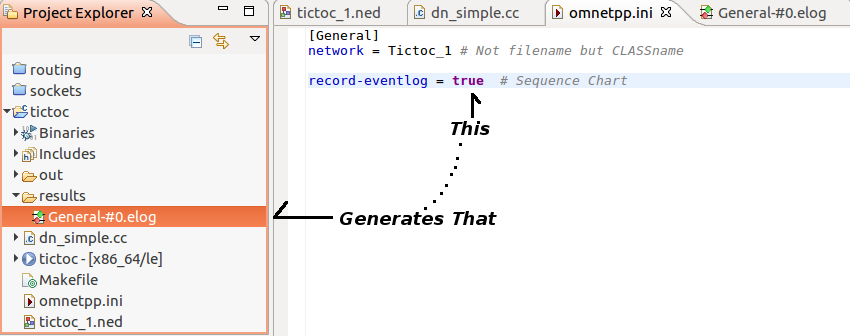
\includegraphics[width=\textwidth]{charting1.png}

        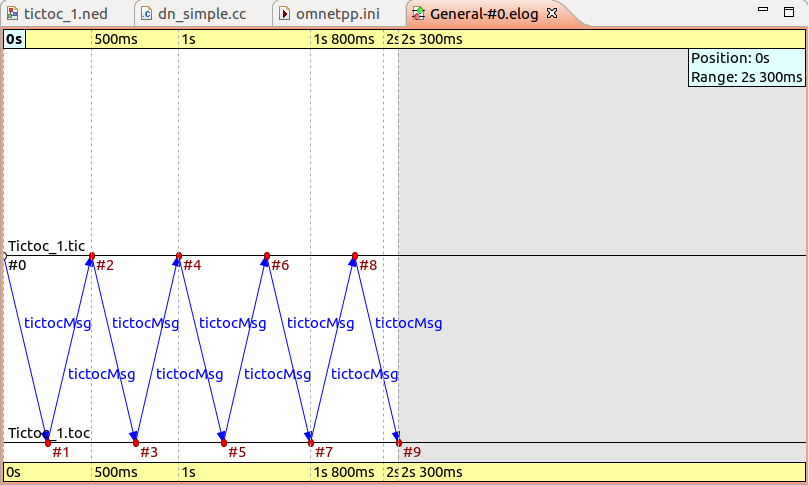
\includegraphics[width=\textwidth]{charting2.png}


    \end{enumerate}
\end{document}